\documentclass[10pt, a4paper]{article}
\usepackage{lrec}
%\usepackage{multibib}
%\newcites{languageresource}{Language Resources}
\usepackage{graphicx}
\usepackage{tabularx}
\usepackage{soul}
% for eps graphics

\usepackage{epstopdf}
\usepackage[latin1]{inputenc}
\usepackage{xspace}
\usepackage{booktabs}
\usepackage{hyperref}
\usepackage{xstring}

\newcommand{\secref}[1]{\StrSubstitute{\getrefnumber{#1}}{.}{ }}

\newcommand{\refexp}[1]{\textsl{#1}}
\newcommand{\word}[1]{\textsl{#1}}
\newcommand{\cat}[1]{\textsc{#1}}
\newcommand{\vgenome}{VisualGenome\xspace}
\newcommand{\vg}{VG\xspace}
\newcommand{\ra}{$\rightarrow$}
\newcommand{\referit}{ReferIt\xspace}
\newcommand{\refcoco}{RefCOCO\xspace}
\newcommand{\refcocop}{RefCOCO+\xspace}
\newcommand{\flickr}{Flickr30k Entities\xspace}

\newcommand{\sz}[1]{\textcolor{blue}{\emph{//sz: #1//}}}
\newcommand{\gbt}[1]{\textcolor{orange}{\emph{//g: #1//}}}
\newcommand{\cs}[1]{\textcolor{green!60!black}{\emph{//cs: #1//}}}

\title{Do resources in Language \& Vision favour the study of linguistic variation? \\ \vspace*{.5\baselineskip} A survey and a new collection of Object Naming data}

\name{Author1, Author2, Author3}

\address{Affiliation1, Affiliation2, Affiliation3 \\
         Address1, Address2, Address3 \\
         author1@xxx.yy, author2@zzz.edu, author3@hhh.com\\
         \{author1, author5, author9\}@abc.org\\}


\abstract{
blabla \\ \newline \Keywords{keyword1, keyword2,
keyword3} }

\begin{document}

\maketitleabstract

\section{Introduction}

Generally, research in Language \& Vision (L\&V) is interested in modeling how speakers \textit{naturally} name, refer to or talk about visual objects and scenes, in contrast to predicting abstract object labels as e.g.\ in Computer Vision.
This typically entails that data collections and models need to account for linguistic variation, as there can hardly ever be a single ground-truth utterance when describing or referring to visual entities. 
An indeed, variation has been accounted for in the modeling and evaluation of certain L\&V tasks like image captioning \cite{vedantam2015cider,Bernardietal:automatic,dai2017towards}.

In principle, the massive data collections now available in L\&V should not only spur computational, application-oriented research aimed at implementing systems for very specific tasks---they should also constitute extremely valuable resources for research aimed at deriving linguistic generalizations about various phenomena related to language grounding, reference and situated interaction which, for a long time, have been investigated mostly in very controlled and small-domain experimental settings, cf. \cite{anderson1991hcrc,fernangen:sigd07,krahmer:2012,takenobu2012rex,zarriess2016pentoref} for some examples of traditional data collections related to reference and grounding.  
In turn, these linguistic generalizations could inform computational modeling, architecture design and future data collections.
However, so far, studies that have tested linguistic hypotheses on large-scale L\&V resources have been relatively rare. 

In this paper, we take a look at object naming, a core phenomenon that occurs in virtually every L\&V task and is, at the same time, subject of ongoing research in language grounding and pragmatics. 
We take stock of existing data sets that provide names for objects in real-world images. We contribute a new dataset, ManyNames, that contains 36 crowd-sourced names for 25K instances from \vg.

\section{Background}

\subsection{Object Naming as a Linguistic Phenomenon}

The act of naming an object amounts to that of picking out a nominal to be employed to refer to it (e.g., ``the \refexp{dog}'', ``the white \refexp{dog} to the left'').
Since an object is simultaneously a member of multiple categories (e.g., a young \refexp{beagle} is at once a \cat{dog}, a \cat{beagle}, an \cat{animal}, a \cat{puppy} etc.), all the various names that lexicalize these constitute a valid alternative, meaning that the same object can be named with more or less \textbf{specific names} \cite{brown1958shall,murphy2004big}. 
Seminal work on concepts by Rosch suggests that object names typically exhibit a preferred level of specificity called the \textbf{entry-level}. This typically corresponds to an intermediate level of specificity, i.e., \textbf{basic level} (e.g, \refexp{bird}, \refexp{car}) \cite{rosch1976basic}, as opposed to more generic (i.e., \textbf{super-level}; e.g., \refexp{animal}, \refexp{vehicle}) or specific categories (i.e., \textbf{sub-level}; e.g., \refexp{sparrow}, \refexp{convertible}). However, less prototypical members of basic-level categories tend to be instead identified with sub-level categories (e.g., a \cat{penguin} is typically called a \refexp{penguin} and not a \refexp{bird}) \cite{jolicoeur1984pictures}. 
%This out-of-context preference towards a certain taxonomic level is often referred to as \textbf{lexical availability}. 
While the traditional notion of entry-level categories suggests that objects tend to be named by a \refexp{single} preferred concept, research on pragmatics has found that speakers are flexible in  
%with respect to the chose level of specificity. 
their choice of the level of specificity. 
Scenarios where multiple objects (of the same category) are present induce a pressure for generating names which uniquely identify the target \cite{olson1970language}, such that sub-level names can be systematically elicited in these cases %\cite{rohde2012communicating} \cite{graf2016animal}. 
\cite{rohde2012communicating}\cite{graf2016animal}.
For example, in presence of more than one dog, the name \textsl{dog} is ambiguous and a sub-level category (e.g., \textsl{rottweiler}, \textsl{beagle}) is more informative and potentially preferred by speakers, though additional factors such as cost or saliency also come into play \cite{graf2016animal}\cite{clark1983common}.

\subsection{Modeling Object Naming}

Though names are prominent in referring expressions, investigated a lot in natural language generation \cite{dale:1995}, this area has focused mostly on the selection of attributes % rather than on determining the referent's name 
\cite{krahmer:2012}. 
\newcite{Ordonez:2016} takes up the notion of entry-level categories \cite{rosch1976basic} and transfers an object's predicted fine-grained label to its name using text corpus statistics.
% extend object recognition to naming, taking up the notion of entry-level categories \cite{rosch1976basic}.
%Their model predicts classifies objects into fine-grained categories and then predicts a WordNet synset for retrieving the name, based on frequencies in a text corpus. 
 \newcite{zarriess-schlangen:2017} learn a naming model on referring expressions and real-world images, but focus on combining visual and distributional information. 
 Recent experimental work on reference found that the specificity of a name is dependent on the taxonomic relatedness of other objects in context

\subsection{Relevant Resources}

justify the following selection of resources....

\begin{table*}
\centering
\begin{tabular}{lrrrrr}
\toprule
                         &   RefCoco &  Flickr30k &           VG &      VGmn &        MN \\
\midrule
                  \# objects & 50.000 & 243.801 & 3.781.232 & 25.223 & 25.315 \\
                naming vocab size &  5.004 &  10.423 &   105.441 &  1.061 &  7.970 \\
     av. annotations/object &      2.84 &       2.30 &         1.69 &      7.24 &     35.30 \\
 \% objects with n types $>$ 1 &      0.68 &       0.29 &         0.02 &      0.05 &      0.93 \\
           av. types/object &      1.88 &       1.38 &         1.02 &      1.08 &      5.70 \\
\bottomrule
\end{tabular}
\caption{Overview statistics for different data sets containing object naming data}
\end{table*}



\section{Survey: Object Naming in L\&V resources}


\subsection{Visual Genome}

\vg \cite{krishna2016visualgenome} is one of the most densely and richly annotated resources currently available in L\&V. In the following, we will focus on describing aspects immediately relevant to object naming only, while many other annotations are available as well (e.g. questions, paragraphs, etc.)

\paragraph{Collection and annotation procedure}

\vg aims to provide a full set of descriptions of the scenes which images depict in order to spur complete scene understanding. 
The data collection followed a complex procedure, involving many different rounds of annotation. The first round of the procedure, and the basic backbone for the further rounds, is a collection of region-based descriptions: workers were asked to describe regions in the image and draw boxes around the corresponding area in the image. In this stage, workers were encouraged to annotate 
In a second independent round (involving new workers), annotators were then asked to process the region descriptions by (i) marking the object names contained in the region description, and (ii) drawing a tight box around the corresponding region. As different region descriptions would potentially mention the same objects, each worker was shown a list of previously marked objects and encouraged to select on existing object rather than annotating a new one.


\begin{figure}
\begin{center}
%\fbox{\parbox{6cm}{
%This is a figure with a caption.}}
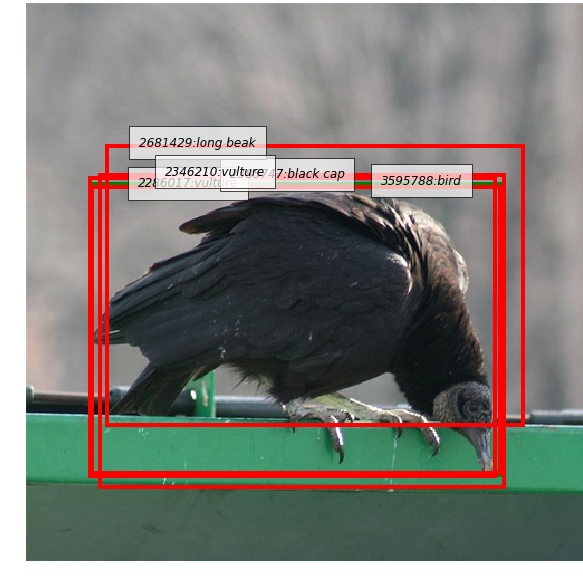
\includegraphics[scale=0.4]{figures/vulture.png} 
\begin{tabular}{lp{6cm}}
object id & linked region descriptions\\
\hline
3595788 & the \textbf{bird} is black in color, nose of the \textbf{bird}, a \textbf{bird} relaxing in stand, small white beak of \textbf{bird}, large black talon of \textbf{bird}, a \textbf{bird} on a green pole, a green bar under \textbf{bird}, black \textbf{bird} on green rail, small black eye of \textbf{bird}\\
2286017 & large black \textbf{vulture} on fence, a vulture on bar\\
2385747 & small white beak of \textbf{bird}\\
2681429 & a semi \textbf{long beak}\\  
2346210 & a black and gray \textbf{vulture}\\
 \end{tabular}
\caption{Bounding boxes, names and region descriptions for an object in VisualGenome}
\label{fig:bird}
\end{center}
\end{figure}

\paragraph{Example}

Figure \ref{fig:bird} shows an example image from VisualGenome, and some of its object annotations. This illustrates that there is only a partial linking of objects that are mentioned across different region descriptions, i.e.\ the identity of objects cannot be established based on the annotation. for a given object and its bounding box, there might be different region descriptions and names associated with it.

\paragraph{Discussion}
\begin{itemize}
\item advantages: exhaustive annotations of all/most objects in the image, variable region descriptions and possibly object names
\item disadvantages: object linking is partial due to bottom-up annotation procedure
\end{itemize}

\subsection{\refcoco and \refcocop}
Both datasets use the \referit\cite{Kazemzadeh2014} game for collecting referring expressions (RE) for natural objects in real-world images, and are built on top of the MS COCO \cite{mscoco}, 
%The latter provides five captions for each of  $300k$~images, spanning $80$~of the COCO categories.  
%However, the COCO region-level (object) annotations are not linked to the captions.
a dataset of images of natural scenes of $91$~common object categories (e.g.,~\cat{dog, pizza, chair}). 
The REs were collected via crowdsourcing in a two-player reference game designed to obtain REs uniquely referring to the target object. 
Specifically, a director and a matcher are presented with an image, and the director produces a RE for an outlined target object in the image. 
The matcher must click on the object he thinks the RE refers to. % (For more details on the datasets see \cite{Yu2016}). 
REs in \refcoco/+ were collected under the constraints that (i) all images contain at least two objects of the same category (80 COCO categories), which prompts the players to avoid the mere object category as RE, and (ii) in \refcocop the players must not use location words, urging them to refer to the appearance of objects. 
%Another critical property of the data is that, (iii), not all objects in an image were annotated with REs, may it due to the frequency constraint~(i), or due to the object not being part of the 80 COCO categories. 

\begin{itemize}
     		\item[(1)] \textbf{Specific categories}: not available, the $80$~COCO categories tend to be entry-level categories and are not linked to the ImageNet taxonomy (e.g.,~\cat{bird, person, car, bus})
		\item[(2)] \textbf{Exhaustive annotations}: not available, as not all objects were annotated with REs and corresponding categories
		   \item[(3)] \textbf{Natural names}: available, though it is unclear how the additional constraints in RefCoco+ impact on the naturalness of object naming
\end{itemize}

\paragraph{Analysis} We parse REs in \refcoco with the Stanford Dependency Parser and extract the nominal heads. We map these names to their most frequent sense/synset in WordNet.
We hypothesize that the distance of a name's synset to the root node (\cat{entity}) relates to its specificity.
We estimate this distance as the minimal path length of all synsets of a word  to the root node.
Table \ref{tab:specnames} shows the estimated levels of specificity for object names in the \refcoco data set.
We observe distances to the root between 2 and 17, meaning that there is a much more fine-grained distinction of levels than the three-way classification adopted in \cite{graf2016animal}.
Unfortunately, the levels of specificity predicted by WordNet do not seem to reflect linguistic intuitions, e.g.\ \refexp{elephant} is predicted to be more specific than \refexp{panda}.
At the same time, this overview clearly suggests that object names in \refcoco do not only comprise entry-level categories, but also very general (\refexp{thing}) and very specific names (\refexp{ox}).

\begin{table*}
\centering
\setlength{\tabcolsep}{2pt}
\begin{small}
\begin{tabular}{rrl|rrl}
\toprule
 spec. &  rel.freq. &                          top 5 names & spec. &  rel.freq. &                          top 5 names \\
\midrule
           2 &   $<$ 0.01 &       \tiny                  thing,things & 10 &   0.05 &   elephant,couch,truck,vase,suitcase \\
           3 &   $<$ 0.01 &    object,group,set,substance,objects & 11 &   $<$ 0.01 &    motorcycle,clock,mom,dad,scissors \\
           4 &   0.14 &           man,person,piece,head,part & 12 &   $<$ 0.01 &  oven,airplane,suv,taxi,refrigerator  \\
           5 &   0.10 &       player,glass,baby,front,corner & 13 &   $<$ 0.01 &    laptop,fridge,canoe,orioles,pigeon \\
           6 &   0.21 &              woman,girl,kid,boy,bowl & 14 &   $<$ 0.01 &   panda,freezer,penguin,rooster,rhino \\
           7 &   0.25 &            guy,right,chair,lady,bear & 15 &   0.03 &    zebra,giraffe,zebras,giraffes,deer \\
           8 &   0.11 &           horse,bus,cow,pizza,batter & 16 &  $ <$ 0.01 &       bison,mooses,orang,elks,sambar \\
           9 &   0.09 &         shirt,car,bike,donut,catcher & 17 &   $<$ 0.01 &           ox,cattle,gnu,mustang,orca \\          
\bottomrule
\end{tabular}\caption{Levels of specificity for naming choices in RefCOCO: for each level (distance between name and WordNet root), relative frequency and 5 most frequent names are shown}
\label{tab:specnames}
\end{small}
\label{tab:specnames}
\end{table*}


\subsection{Flickr30k Entities}
The \flickr dataset \cite{plummer2015flickr30kentities}\footnote{Available at  \url{web.engr.illinois.edu/~bplumme2/Flickr30kEntities}}  augments Flickr30k, a dataset of 30k~images and five sentence-level captions for each of the images, with region-level annotations. 
Specifically, mentions of the same entities across the five captions of an image are linked to the bounding boxes of the objects they refer to. 
The dataset was designed to advance image description generation and phrase localization in particular (e.g.,~\cite{rohrbach2016grounding,plummer2017phrase,yeh2018unsupervised}). 

By design, \flickr can be used to study the way people refer to individual entities in an image depending on the situation the speakers describe and,  
in contrast to \refcoco/+, the production of entity mentions did not underlie any constraints. 
On the other hand, it is less suited for referring expression generation since mentions in isolation of their linguistic context may not uniquely identify the referred object. 

\begin{itemize}
     		\item[(1)] \textbf{Specific categories}: are not available, object categories tend to be even less specific than those of COCO (e.g.,~\cat{people, animals, bodyparts, clothing}), or are abstract (\cat{other, scene})
		\item[(2)] \textbf{Exhaustive annotations}: are not available
		   \item[(3)] \textbf{Natural names}: are available, though object names might not be fully discriminative (as in REs; e.g.,~both animals in the right-most image in Fig.~\ref{fig:graf_genome} are named \refexp{dog})

\end{itemize}



\section{Conclusion}

Your submission of a finalised contribution for inclusion in the LREC
proceedings automatically assigns the above-mentioned copyright to ELRA.


\section{Acknowledgements}

Place all acknowledgements (including those concerning research grants and
funding) in a separate section at the end of the article.

\section{Bibliographical References}
\label{main:ref}

\bibliographystyle{lrec}
\bibliography{naming}


%\section{Language Resource References}
%\label{lr:ref}
%\bibliographystylelanguageresource{lrec}
%\bibliographylanguageresource{lrec2020W-xample}

\end{document}
